\documentclass[tikz,border=10pt]{standalone}
\usepackage{pgfplots}
\pgfplotsset{compat=1.18}
\usepackage{amsmath,amssymb,bm}
\definecolor{darkbg}{HTML}{1a1a1a}
\definecolor{lightfg}{HTML}{e8e6e3}
\definecolor{accent}{HTML}{7cb87c}
\definecolor{accent2}{HTML}{6aa0b0}
\definecolor{mutedcol}{HTML}{9a9a9a}
\definecolor{bordercol}{HTML}{3d3d3d}
\definecolor{redcol}{HTML}{cc3333}
\definecolor{bluecol}{HTML}{4466cc}
\pagecolor{darkbg}
\color{lightfg}

\usetikzlibrary{arrows.meta}

\begin{document}
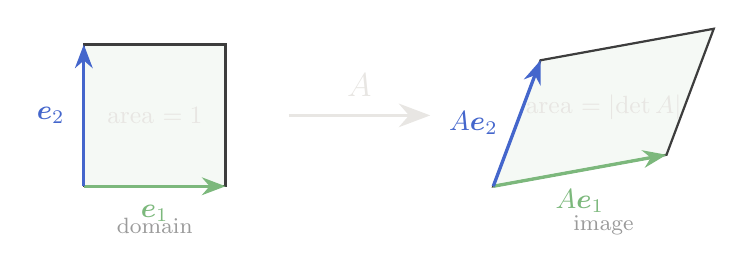
\begin{tikzpicture}

% === LEFT: Unit square (domain) ===
\begin{scope}[shift={(0,0)}]
  \fill[accent, opacity=0.08] (0,0) rectangle (1.8,1.8);
  \draw[bordercol, thick] (0,0) rectangle (1.8,1.8);

  \draw[-{Stealth[length=3mm]}, accent, very thick]
    (0,0) -- (1.8,0) node[midway, below=3pt, accent] {$\bm{e}_1$};
  \draw[-{Stealth[length=3mm]}, bluecol, very thick]
    (0,0) -- (0,1.8) node[midway, left=3pt, bluecol] {$\bm{e}_2$};

  \node[lightfg, font=\small] at (0.9,0.9) {area $= 1$};
  \node[mutedcol, font=\footnotesize] at (0.9,-0.5) {domain};
\end{scope}

% === CENTER: Arrow labeled A ===
\draw[-{Stealth[length=4mm]}, lightfg, very thick]
  (2.6,0.9) -- (4.4,0.9) node[midway, above=3pt, lightfg, font=\large] {$A$};

% === RIGHT: Parallelogram (image) ===
\begin{scope}[shift={(5.2,0)}]
  \pgfmathsetmacro{\ax}{2.2}
  \pgfmathsetmacro{\ay}{0.4}
  \pgfmathsetmacro{\bx}{0.6}
  \pgfmathsetmacro{\by}{1.6}

  \fill[accent, opacity=0.08]
    (0,0) -- (\ax,\ay) -- ({\ax+\bx},{\ay+\by}) -- (\bx,\by) -- cycle;
  \draw[bordercol, thick]
    (0,0) -- (\ax,\ay) -- ({\ax+\bx},{\ay+\by}) -- (\bx,\by) -- cycle;

  \draw[-{Stealth[length=3mm]}, accent, very thick]
    (0,0) -- (\ax,\ay) node[midway, below=3pt, accent] {$A\bm{e}_1$};
  \draw[-{Stealth[length=3mm]}, bluecol, very thick]
    (0,0) -- (\bx,\by) node[midway, left=3pt, bluecol] {$A\bm{e}_2$};

  \node[lightfg, font=\small] at ({(\ax+\bx)/2},{(\ay+\by)/2}) {area $= |\!\det A|$};
  \node[mutedcol, font=\footnotesize] at ({(\ax+\bx)/2},-0.5) {image};
\end{scope}

\end{tikzpicture}
\end{document}
